\documentclass[main.tex]{subfiles}
\begin{document}

% ── Part 1: Theory ─────────────────────────────────────────────────────
\section{Callaway \& Sant'Anna (2021)}

% ── A1: Bridge from Block 0 ─────────────────────────────────────────────
\begin{frame}{Where We Left Off: The TWFE Problem}

  \textbf{Block 0 showed:} TWFE with staggered adoption is a weighted
  average of all possible 2$\times$2 DiDs, and the weights on those
  2$\times$2 \emph{blocks} are all positive (Goodman-Bacon).

  \medskip
  (Block 2 revisits the same designs through dCH's cell-level weights, where
  some already-treated cells get \alert{negative} weight --- the central issue
  once treatment is non-binary or non-absorbing.)

  \medskip
  The root cause: TWFE uses \alert{already-treated units as controls}
  for later-treated units; if their effects change over time, that change
  is subtracted and biases $\hat{\beta}$.

  \bigskip
  \textbf{The fix requires three things:}
  \begin{enumerate}
    \item Build every comparison using only \emph{clean} control units
    \item Allow treatment effects to differ across groups and over time
    \item Aggregate the results into summaries we can interpret
  \end{enumerate}

  \bigskip
  \textbf{This block:} Callaway \& Sant'Anna (2021) deliver all three.\\
  \textit{Use case: binary, absorbing, staggered treatment with
    many treated units.}

\end{frame}

% ── A2: The key object — ATT(g,t) ───────────────────────────────────────
\begin{frame}{The Key Idea: Think in Cohorts}

  \textbf{Instead of one $\hat{\beta}$, estimate one ATT per
  (cohort, calendar year) cell.}

  \bigskip
  \begin{columns}[T]
    \begin{column}{0.50\textwidth}
      \textbf{Define:}
      \begin{itemize}
        \item $g$ = the year a unit is \emph{first} treated
          (its ``cohort'')
        \item $t$ = the calendar year of measurement
      \end{itemize}

      \bigskip
      \begin{block}{Group-Time ATT}
        \[
          \text{ATT}(g,t) = E\!\left[\,Y_t(g) - Y_t(0)\;\middle|\;G=g\,\right]
        \]
      \end{block}

      \medskip
      Average treatment effect for cohort $g$ at time $t$,
      averaged only over units in that cohort.
    \end{column}
    \begin{column}{0.46\textwidth}
      \textbf{A grid, not a single number:}
      \begin{itemize}
        \item One ATT$(g,t)$ per (cohort, period) cell, $t \ge 2$
          $\Rightarrow$ a $G \times (T{-}1)$ grid
        \item Cells with $t < g$: \emph{pre-treatment}, $\approx 0$
          under no anticipation and parallel trends
        \item Cells with $t \geq g$ are the effects of interest
      \end{itemize}

      \medskip
      \begin{block}{No restriction imposed}
        Effects may differ \emph{across cohorts} and
        \emph{over time}. TWFE forces them into one $\hat\beta$;
        C\&S keeps them separate.
      \end{block}
    \end{column}
  \end{columns}

\end{frame}

% ── A2b: The ATT(g,t) grid, concretely ──────────────────────────────────
\begin{frame}{The ATT$(g,t)$ Grid, Made Concrete}

  \textbf{Each box is one cell $\text{ATT}(g,t)$:} row $=$ cohort (year first
  treated), column $=$ calendar year. Three cohorts plus a never-treated group:

  \smallskip
  \begin{center}
  \begin{tikzpicture}[font=\footnotesize,
    cell/.style={draw=white, line width=1pt, minimum width=1.85cm,
                 minimum height=0.78cm, inner sep=1pt},
    pre/.style={cell, fill=MidBlue!18},
    post/.style={cell, fill=AlertRed!20},
    ctrl/.style={cell, fill=black!8},
    hd/.style={cell, fill=DarkBlue, text=white, font=\footnotesize\bfseries},
    rl/.style={anchor=east, font=\footnotesize\bfseries}]
    \node[hd] at (0,3.12){2004}; \node[hd] at (1.85,3.12){2005};
    \node[hd] at (3.7,3.12){2006}; \node[hd] at (5.55,3.12){2007};
    \node[rl] at (-1.05,2.34){treated 2004};
    \node[rl] at (-1.05,1.56){treated 2006};
    \node[rl] at (-1.05,0.78){treated 2007};
    \node[rl] at (-1.05,0){never treated};
    % g2004: all post (no pre -- treated from start of window)
    \node[post] at (0,2.34){ATT}; \node[post] at (1.85,2.34){ATT};
    \node[post] at (3.7,2.34){ATT}; \node[post] at (5.55,2.34){ATT};
    % g2006: pre, pre, ATT, ATT
    \node[pre] at (0,1.56){pre}; \node[pre] at (1.85,1.56){pre};
    \node[post] at (3.7,1.56){ATT}; \node[post] at (5.55,1.56){ATT};
    % g2007: pre, pre, pre, ATT
    \node[pre] at (0,0.78){pre}; \node[pre] at (1.85,0.78){pre};
    \node[pre] at (3.7,0.78){pre}; \node[post] at (5.55,0.78){ATT};
    % never: control
    \node[ctrl] at (0,0){--}; \node[ctrl] at (1.85,0){--};
    \node[ctrl] at (3.7,0){--}; \node[ctrl] at (5.55,0){--};
  \end{tikzpicture}
  \end{center}

  \smallskip
  {\footnotesize
  \colorbox{AlertRed!20}{\strut\,ATT\,} effect ($t\ge g$) \quad
  \colorbox{MidBlue!18}{\strut\,pre\,} pre-treatment check ($t<g$, $\approx 0$) \quad
  \colorbox{black!8}{\strut\,--\,} never-treated control}

\end{frame}

% ── A3: Staggered adoption assumption ───────────────────────────────────
\begin{frame}{Assumption 1: Staggered (Absorbing) Treatment}

  \textbf{Once treated, always treated:}
  \[
    D_{i1} = 0 \quad\text{and}\quad D_{i,t-1} = 1 \;\Rightarrow\; D_{it} = 1
    \quad (t = 2,\dots,T)
  \]

  \medskip
  Nobody is treated in period 1 (such units are dropped); $G_i = g$ if
  first treated in $g$.

  \bigskip
  \begin{columns}[T]
    \begin{column}{0.48\textwidth}
      \textbf{Why this matters:}
      \begin{itemize}
        \item Each unit belongs to exactly one cohort
        \item Pre-treatment periods of a cohort are clean
        \item Placebo ``pseudo'' $\text{ATT}(g,t)$ for $2 \le t < g$:
          $\approx 0$ under PT and no anticipation
      \end{itemize}
    \end{column}
    \begin{column}{0.48\textwidth}
      \textbf{Common examples:}
      \begin{itemize}
        \item Minimum wage laws (state adoption)
        \item ACA Medicaid expansion
        \item Environmental regulations
        \item No-fault divorce laws
      \end{itemize}

      \medskip
      \alert{Not satisfied:} treatment that can be reversed or
      is continuous. $\to$ Block 2.
    \end{column}
  \end{columns}

\end{frame}

% ── A4: Parallel trends — two versions ──────────────────────────────────
\begin{frame}{Assumption 2: Parallel Trends (C\&S Assumptions 4--5)}

  \textbf{Unconditional version} (simplest), for each cohort $g$ and each $t \ge g$:
  \[
    E\!\left[Y_t(0) - Y_{t-1}(0)\;\middle|\;G=g\right]
    = E\!\left[Y_t(0) - Y_{t-1}(0)\;\middle|\;\text{control group}\right]
  \]

  Absent treatment, cohort $g$ moves in parallel with its controls from
  $g{-}1$ on.

  \smallskip
  \textit{Identification uses the \textbf{long difference} relative to
  $g{-}1$ (the cohort's last pre-treatment year), not period-by-period
  first differences --- so $g{-}1$ is the natural baseline (relative
  time $e=-1$).}

  \medskip
  \textbf{Conditional version} (more flexible), for each $g$ and $t \ge g$:
  \[
    E\!\left[Y_t(0) - Y_{t-1}(0)\;\middle|\;X,\, G=g\right]
    = E\!\left[Y_t(0) - Y_{t-1}(0)\;\middle|\;X,\, \text{control group}\right]
  \]

  Use it when pre-treatment $X$ that drive the trend of $Y(0)$ differ
  across groups.

  \medskip
  \begin{alertblock}{Why this matters}
    The conditional version is what motivates the doubly-robust estimator.
  \end{alertblock}

\end{frame}

% ── A5: Control groups ───────────────────────────────────────────────────
\begin{frame}{Who Is the Control Group?}

  C\&S offers two \alert{clean} options. The choice matters for both
  credibility and power.

  \bigskip
  \begin{columns}[T]
    \begin{column}{0.48\textwidth}
      \begin{block}{Never-treated units}
        Units that are never treated throughout the sample.\\[6pt]
        \textbf{Pro:} most stable counterfactual\\
        \textbf{Con:} may be too few; may differ systematically
      \end{block}
    \end{column}
    \begin{column}{0.48\textwidth}
      \begin{block}{Not-yet-treated units}
        Units that will eventually be treated, but have not been
        treated \emph{yet} at time $t$.\\[6pt]
        \textbf{Pro:} more comparison units; arguably more similar\\
        \textbf{Con:} imposes restrictions on pre-trends across
        cohorts
      \end{block}
    \end{column}
  \end{columns}

  \bigskip
  \textbf{What is \emph{excluded} in both cases:}
  already-treated units --- the source of TWFE bias.

\end{frame}

% ── A6: Doubly robust estimator ─────────────────────────────────────────
\begin{frame}{The Doubly Robust Estimator}

  For each $(g, t)$ cell, C\&S identifies ATT using one of three
  equivalent approaches:

  \begin{enumerate}
    \item \textbf{Outcome regression (OR):} model the controls' change
      $E[Y_t - Y_{g-1}\,|\,X]$ and impute it for cohort $g$
    \item \textbf{IPW:} re-weight control units by the odds
      $p_g(X)/(1-p_g(X))$ of being in cohort $g$ rather than control
    \item \textbf{Doubly robust (DR):} combine both
  \end{enumerate}

  \medskip
  \begin{alertblock}{Why doubly robust?}
    Consistent if \emph{either} the propensity-score model \emph{or} the
    outcome regression is correctly specified --- not necessarily both.
  \end{alertblock}

  \medskip
  \textbf{In practice:} the doubly-robust estimator is the default ---
  and the authors' recommendation.

  \smallskip
  \textbf{Required: overlap.} $P(G_g{=}1) > \varepsilon$ and
  $p_{g,t}(X) < 1{-}\varepsilon$ for almost every $X$. As $p \to 1$,
  IPW weights $p/(1{-}p)$ blow up and IPW/DR become very imprecise.

\end{frame}

% ── A7: Aggregation ──────────────────────────────────────────────────────
\begin{frame}{From ATT$(g,t)$ to Summaries: Aggregation}

  With $G$ cohorts and $T$ periods, you have up to $G \times (T{-}1)$
  estimates (period 1 is only a base period).
  Aggregate them into one of four summaries:

  \bigskip
  \begin{tabular}{lll}
    \toprule
    \textbf{Summary} & \textbf{Parameter} & \textbf{Use when\ldots} \\
    \midrule
    Event study & $\theta_{es}(e)$ &
      Show dynamics; assess pre-trends \\
    \addlinespace
    Group-specific & $\theta_{sel}(g)$ &
      Compare early vs.\ late adopters \\
    \addlinespace
    Calendar time & $\theta_{c}(t)$ &
      Effects in a specific period \\
    \addlinespace
    Overall ATT & $\theta_O$ &
      Single number for abstract/table \\
    \bottomrule
  \end{tabular}

  \bigskip
  \textbf{Key:} all four are weighted averages of the same
  ATT$(g,t)$ grid --- they answer different questions, not
  different models.

\end{frame}

% ── A7b: Formal estimands ─────────────────────────────────────────────────
\begin{frame}{Aggregation: The Formal Estimands}

  All four summaries are weighted averages of the ATT$(g,t)$ grid
  (Callaway \& Sant'Anna 2021):

  \medskip
  \begin{align*}
    \theta_{es}(e)  &= \textstyle\sum_g \mathbf{1}\{g{+}e \le T\}\;
        P(G{=}g \mid G{+}e \le T)\; \text{ATT}(g, g{+}e)
        && \text{\small event study}\\[2pt]
    \theta_{sel}(g) &= \tfrac{1}{T-g+1}\textstyle\sum_{t \ge g} \text{ATT}(g,t)
        && \text{\small group-specific}\\[2pt]
    \theta_{c}(t)   &= \textstyle\sum_g \mathbf{1}\{t \ge g\}\;
        P(G{=}g \mid G \le t)\; \text{ATT}(g,t)
        && \text{\small calendar}\\[2pt]
    \theta_{O}      &= \textstyle\sum_g \theta_{sel}(g)\,P(G{=}g \mid G \le T)
        && \text{\small overall}
  \end{align*}

  \medskip
  \begin{alertblock}{Two ways to weight the ``overall'' effect}
    $\theta_O^{\,sel}$ averages \emph{within} groups first, then across
    groups --- the authors' preferred summary.
    $\theta_O^{\,W}$ weights every post-treatment cell by group size,
    putting more weight on early-treated groups.
    In general they differ; they coincide when every cohort has the same
    $\theta_{sel}(g)$ (for example, under homogeneous effects).
  \end{alertblock}

\end{frame}

% ── A7c: estimand deep-dive (one per parameter) ──────────────────────────
\begin{frame}{Event Study $\theta_{es}(e)$: Effect by Time Since Treatment}

  \begin{description}[Averages]
    \item[Question] How does the effect evolve with exposure length $e = t-g$?
    \item[Averages] the cells $\text{ATT}(g,g{+}e)$ at horizon $e$, weighted by
      cohort size. $e{=}0$ is the on-impact effect; $e{<}0$ is pre-treatment.
    \item[Use it] the headline plot --- trace whether effects build, fade, or persist.
    \item[\color{AlertRed}Gotcha] the $e{<}0$ points are \emph{not} effects: they
      are the parallel-trends check and should sit near $0$. Read the whole path,
      not a single horizon.
  \end{description}

\end{frame}

% ── A8: Event study intuition ────────────────────────────────────────────
\begin{frame}{The Event Study Plot}

  \textbf{Most useful output from C\&S:} the dynamic aggregation
  $\theta_{\mathit{es}}(e)$ --- the average effect $e$ periods after first
  treatment.

  \medskip
  \begin{columns}[T]
    \begin{column}{0.50\textwidth}
      \begin{tikzpicture}[scale=0.75]
        \draw[->] (-3.5,0) -- (3.2,0)
          node[right,font=\tiny] {$e$};
        \draw[->] (0,-1.2) -- (0,0.5)
          node[above,font=\tiny] {ATT};
        % zero line
        \draw[dashed,gray!70] (-3.5,0) -- (3.5,0);
        % treatment onset marker
        \draw[dashed,DarkBlue] (0,-1.2) -- (0,0.5);
        \node[below,DarkBlue,font=\tiny] at (0,-1.2) {treatment};
        % pre-treatment: near zero
        \foreach \x/\y in {-3/0.05,-2/-0.02,-1/0.03}{
          \fill[MidBlue] (\x,\y) circle (2.5pt);
          \draw[MidBlue,thick] (\x,\y-0.15) -- (\x,\y+0.15);
        }
        % post-treatment: growing negative
        \foreach \x/\y in {0/-0.02,1/-0.35,2/-0.65,3/-0.85}{
          \fill[AlertRed] (\x,\y) circle (2.5pt);
          \draw[AlertRed,thick] (\x,\y-0.15) -- (\x,\y+0.15);
        }
        % labels
        \node[MidBlue,font=\tiny,text width=2cm,align=center] at (-2,-0.45)
          {Pre-treatment:\\should be $\approx 0$};
        \node[AlertRed,font=\tiny,text width=2cm,align=center] at (2,-1.1)
          {Post-treatment:\\growing effect};
      \end{tikzpicture}

      \vspace{0.5cm}
      \footnotesize
      \textbf{Confidence intervals:} use \textbf{simultaneous} (joint)
      bands --- wider than pointwise, correct for reading the whole
      pre-trend path as one joint test.
    \end{column}
    \begin{column}{0.44\textwidth}
      \small
      \textbf{Reading the plot:}
      \begin{itemize}
        \item $e < 0$: pre-treatment. Should be $\approx 0$ --- an
          honest pre-trends check (but low power, and conditioning on
          passing it distorts inference, Roth 2022).
        \item $e \geq 0$: post-treatment effects. Slope shows
          whether the effect grows, fades, or is constant.
      \end{itemize}

      \medskip
      \alert{Unlike TWFE:} pre-trends here are not contaminated
      by heterogeneous post-treatment effects.
    \end{column}
  \end{columns}

\end{frame}

\begin{frame}{Group Effect $\theta_{sel}(g)$: One Cohort's Average}

  \begin{description}[Averages]
    \item[Question] What was the average effect for the cohort first treated at $g$,
      over its post-treatment life?
    \item[Averages] $\text{ATT}(g,t)$ for $t \ge g$, with \emph{equal} weight
      $1/(T{-}g{+}1)$ --- a single cohort, so no group-size weighting.
    \item[Use it] compare \textbf{early vs.\ late adopters}: is the effect larger
      for those treated sooner?
    \item[\color{AlertRed}Gotcha] later cohorts have fewer post-periods, so their
      average covers a \emph{shorter} horizon --- not a like-for-like comparison
      with early cohorts.
  \end{description}

\end{frame}

\begin{frame}{Calendar Effect $\theta_c(t)$: One Year's Average}

  \begin{description}[Averages]
    \item[Question] What was the average effect in calendar year $t$, across
      everyone treated by then?
    \item[Averages] $\text{ATT}(g,t)$ over cohorts with $g \le t$, weighted by
      cohort size $P(G{=}g \mid G \le t)$.
    \item[Use it] when a specific \textbf{period} matters --- a recession, a
      national shock --- and you want the effect in \emph{that} year.
    \item[\color{AlertRed}Gotcha] a later year is not ``longer exposure'': it has
      \emph{more} cohorts treated. Moving across $t$ changes who is included, not
      just the dynamics.
  \end{description}

\end{frame}

\begin{frame}{Overall Effect $\theta_O$: The Single Number}

  \begin{description}[Averages]
    \item[Question] One headline number for the abstract or a summary table.
    \item[Averages] each cohort's own average $\theta_{sel}(g)$ first, then across
      cohorts weighted by size $P(G{=}g \mid G \le T)$ --- the 2$\times$2 ATT analog.
    \item[Use it] the scalar to report \emph{alongside} --- never instead of ---
      the event study.
    \item[\color{AlertRed}Gotcha] it hides all dynamics and cohort heterogeneity:
      a single $-0.03$ can mask effects that grow, fade, or differ sharply by cohort.
  \end{description}

\end{frame}

% ── A9: No-anticipation assumption ──────────────────────────────────────
\begin{frame}{Assumption 3: No Anticipation (C\&S Assumption 3, $\delta=0$)}

  \textbf{Units in cohort $g$ behave as untreated in all periods
  before $g$:}
  \[
    E\!\left[Y_t(g)\;\middle|\;G=g\right]
    = E\!\left[Y_t(0)\;\middle|\;G=g\right]
    \quad \text{for all } t < g
  \]

  \bigskip
  \begin{columns}[T]
    \begin{column}{0.50\textwidth}
      \textbf{In practice, this means:}
      \begin{itemize}
        \item Units did not change behavior before the treatment
          date in anticipation of being treated
        \item Pre-treatment ATT$(g,t)$ are zero under this assumption;
          nonzero pre-period estimates signal a failure of it or of
          parallel trends
      \end{itemize}
    \end{column}
    \begin{column}{0.46\textwidth}
      \textbf{When might it fail?}
      \begin{itemize}
        \item Firms adjust before a law takes effect
        \item States change spending in anticipation of a federal
          matching program
      \end{itemize}

      \medskip
      \textbf{Partial fix:} C\&S allow a \emph{known} anticipation
      window $\delta \geq 0$ (e.g., 1 year): the reference period
      moves to $g-\delta-1$, and parallel trends must then hold over
      more periods.
    \end{column}
  \end{columns}

\end{frame}

% ── A10: When to use C&S vs. alternatives ───────────────────────────────
\begin{frame}{When Is C\&S the Right Choice?}

  \begin{columns}[T]
    \begin{column}{0.48\textwidth}
      \textbf{Use C\&S when:}
      \begin{itemize}
        \item Treatment is \textbf{binary and absorbing}
        \item Many treated units (across multiple cohorts)
        \item You suspect treatment effect \textbf{heterogeneity}
          across cohorts or dynamics over time
        \item You want an honest pre-trends test
        \item Some groups differ on observables $\to$ use covariates
          with the DR estimator
      \end{itemize}
    \end{column}
    \begin{column}{0.48\textwidth}
      \textbf{Use something else when:}
      \begin{itemize}
        \item Treatment is \textbf{non-absorbing / continuous}
          $\to$ Block 2 (de Chaisemartin \& D'H; for a continuous dose,
          Callaway, Goodman-Bacon \& Sant'Anna)
        \item Very few treated units
          $\to$ Block 3 (Synthetic Control)
        \item You are \emph{certain} treatment effects are
          homogeneous and constant $\to$ TWFE recovers the ATT
      \end{itemize}
    \end{column}
  \end{columns}

  \bigskip
  \begin{block}{For the mathematically inclined}
    \footnotesize
    Formal identification results and asymptotic theory:
    Callaway \& Sant'Anna (2021), \textit{Journal of Econometrics}
    225(2), pp.\ 200--230. Doubly-robust estimand derived in
    Sant'Anna \& Zhao (2020).
  \end{block}

\end{frame}

% ── Part 2: Applications ───────────────────────────────────────────────
\section{Applications}

% ── Demo overview ────────────────────────────────────────────────────────
\begin{frame}{Applied Case: Real Data, Reproducible Stata}

  \textbf{One estimator, the full C\&S workflow on real data.}

  \bigskip
  \begin{block}{Minimum wage and teen employment (Callaway \& Sant'Anna 2021)}
    \textbf{Data:} \texttt{mpdta} --- 500 US counties $\times$ 2003--2007\\
    \textbf{Outcome:} log teen employment (\texttt{lemp})\\
    \textbf{Treatment:} state minimum-wage increase; 3 cohorts
    (2004, 2006, 2007) + never-treated\\[4pt]
    \textbf{Why C\&S:} staggered timing across cohorts, with effects that may
    differ by cohort and grow with exposure --- exactly where TWFE's
    forbidden comparisons bite.
  \end{block}

  \bigskip
  \textbf{Roadmap:} estimate the ATT$(g,t)$ grid, then read it through each
  aggregation --- event study $\theta_{es}(e)$, by cohort $\theta_{sel}(g)$,
  by calendar year $\theta_c(t)$, and the overall $\theta_O$.

\end{frame}

% ═══════════════════════════════════════════════════════════════════════
% CASE 1: mpdta — Minimum Wage and Teen Employment
% ═══════════════════════════════════════════════════════════════════════

% ── Case 1: Context ──────────────────────────────────────────────────────
\begin{frame}{Minimum Wage and Teen Employment}

  \textbf{Research question:} did state minimum wage laws reduce
  teen employment?

  \medskip
  \textbf{Why C\&S, not TWFE?}
  \begin{itemize}
    \item State minimum wage laws adopted in different years ---
      three cohorts: 2004, 2006, 2007
    \item TWFE uses already-treated counties as controls for
      later-treated counties --- the forbidden comparison
    \item If employment effects grow with exposure time,
      late cohorts' controls are contaminated by early-cohort
      post-treatment effects
  \end{itemize}

  \medskip
  \textbf{Data structure:}
  \begin{itemize}
    \item \texttt{mpdta}: 500 counties $\times$ 5 years (2003--2007), 2{,}500 obs
    \item Outcome: \texttt{lemp} --- log teen employment per county
    \item Cohort variable: \texttt{first\_treat} $\in \{2004, 2006, 2007, 0\}$
      ($0$ = never treated)
  \end{itemize}

\end{frame}

% ── Case 1: Stata code ───────────────────────────────────────────────────
\begin{frame}[fragile]{Stata: Estimation, Aggregations, TWFE Benchmark}

\lstset{
  language={},
  basicstyle=\tiny\ttfamily,
  keywordstyle=\color{MidBlue},
  commentstyle=\color{gray},
  breaklines=true,
  showstringspaces=false
}

\begin{lstlisting}
* ssc install csdid drdid, replace

use "$datadir/mpdta.dta", clear
xtset county_id year

* Step 1: estimate all ATT(g,t) cells (doubly robust) and save the RIF file
csdid lemp, ivar(county_id) time(year) gvar(first_treat) ///
    method(dripw) notyet saverif(rif_mpdta) replace
* Step 2: aggregations from the saved RIF file -- each is one theta
preserve
use rif_mpdta, clear
csdid_stats simple,   wboot rseed(1234) /* theta_O^W    = -0.040  */
csdid_stats group,    wboot rseed(1234) /* theta_sel(g); theta_O = -0.030 */
csdid_stats event,    wboot rseed(1234) /* theta_es(e): dynamic   */
csdid_stats calendar, wboot rseed(1234) /* theta_c(t):  by year   */
* Step 3: event-study plot
qui csdid_stats event, wboot rseed(1234)
csdid_plot, title("Event Study: Min. Wage and Teen Employment") ///
    xtitle("Periods relative to first treatment")               ///
    ytitle("ATT (log teen employment)")
graph export "$figdir/mpdta_eventstudy.png", replace width(1200)
restore
* Static TWFE benchmark (clustered by county), on mpdta
gen byte treat_post = (first_treat>0 & year>=first_treat)
xtreg lemp treat_post i.year, fe vce(cluster county_id) /* -0.037* */
\end{lstlisting}

  \textbf{Key:} \texttt{method(dripw)} = doubly robust;
  \texttt{notyet} = not-yet-treated controls;
  \texttt{saverif()} = RIF file read by \texttt{csdid\_stats};
  \texttt{wboot} = wild bootstrap SEs.

\end{frame}

% ── Case 1: Figure + interpretation ─────────────────────────────────────
\begin{frame}{Event Study: Dynamic Effects $\theta_{es}(e)$}

  \begin{columns}[T]
    \begin{column}{0.55\textwidth}
      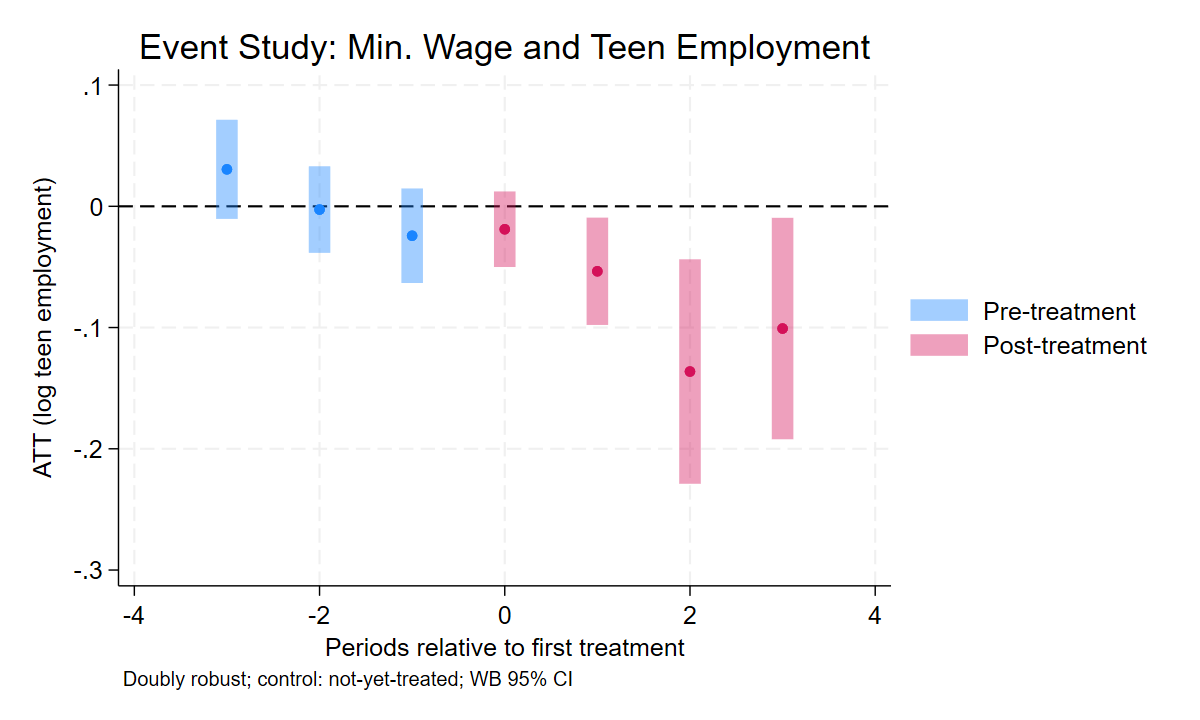
\includegraphics[width=\textwidth]{figures/cs/mpdta_eventstudy.png}
    \end{column}
    \begin{column}{0.42\textwidth}
      \small
      \textbf{Estimand:} $\theta_{es}(e)$ (dynamic).

      \medskip
      \textbf{Pre-trends ($e<0$):} Pre\_avg $=0.001$ (ns);
      $e=-3$: $0.031$ ($p=0.04$). No evidence against PT on
      average (not proof).

      \medskip
      \textbf{Post-treatment:} grows to $\theta_{es}(2)=-0.136$
      log points (2004 only); Post\_avg $=-0.077$.

      \medskip
      \textbf{Overall ($\theta_O^{sel}$):} $-0.030$ (SE 0.012,
      sig at 5\%) --- a $\sim$3\% employment drop.

      \medskip
      \alert{vs.\ static TWFE:} $-0.037$ (sig) on \texttt{mpdta}
      --- close here. The larger gap (TWFE $-0.8\%$ ns vs DR
      with covariates $-3.1\%$) is in the paper's full sample
      (C\&S 2021, Table 3b).
    \end{column}
  \end{columns}

\end{frame}

% ── Case 1: Group ATT code ───────────────────────────────────────────────
\begin{frame}[fragile]{Stata: ATT by Cohort $\theta_{sel}(g)$}

\lstset{
  language={},
  basicstyle=\small\ttfamily,
  keywordstyle=\color{MidBlue},
  commentstyle=\color{gray},
  breaklines=true,
  showstringspaces=false
}

\begin{lstlisting}
* Same estimated model (saved RIF file) -- aggregate by cohort
use rif_mpdta, clear
csdid_stats group, wboot rseed(1234)

csdid_plot, title("ATT by Cohort: Min. Wage and Teen Employment") ///
    xtitle("Treatment cohort")                                     ///
    ytitle("ATT (log teen employment)")
graph export "$figdir/mpdta_group.png", replace width(1200)
\end{lstlisting}

  \medskip
  \textbf{What changes:} \texttt{group} instead of \texttt{event}.
  Same model, different aggregation of the ATT$(g,t)$ grid.

\end{frame}

% ── Case 1: Group ATT ────────────────────────────────────────────────────
\begin{frame}{Effect by Cohort: $\theta_{sel}(g)$}

  \begin{columns}[T]
    \begin{column}{0.55\textwidth}
      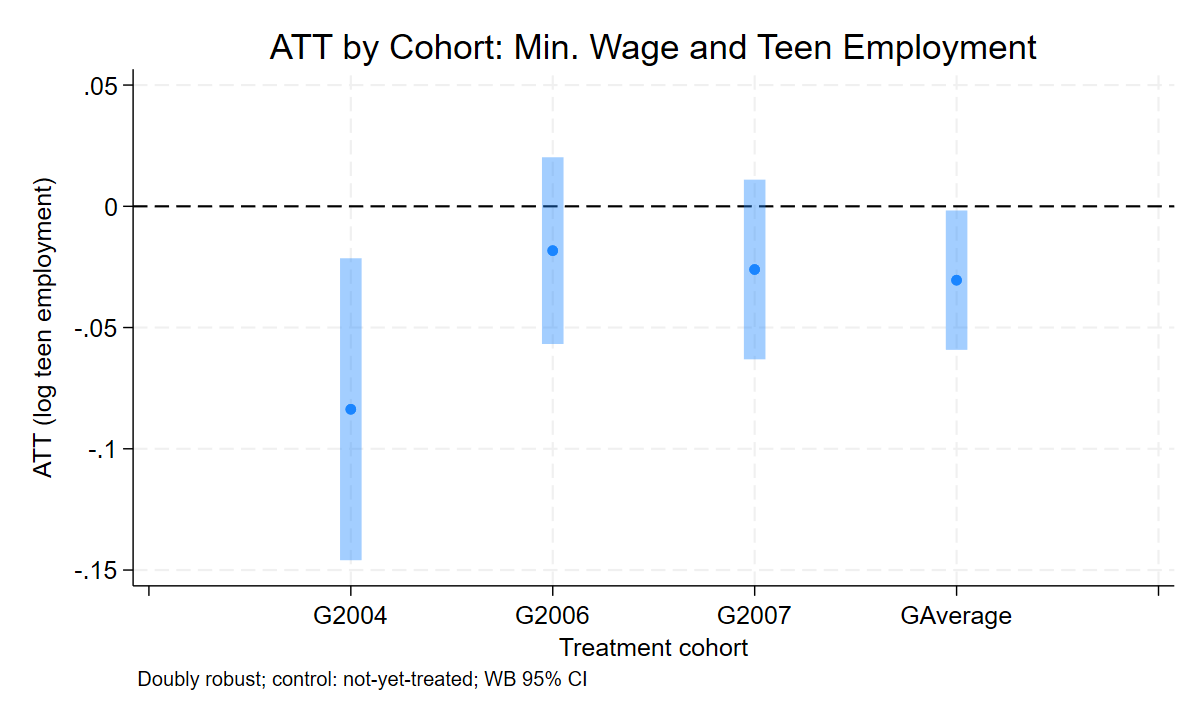
\includegraphics[width=\textwidth]{figures/cs/mpdta_group.png}
    \end{column}
    \begin{column}{0.42\textwidth}
      \small
      \textbf{Estimand: $\theta_{sel}(g)$} --- average effect for each
      cohort over its post-treatment years;
      GAverage $=\theta_O^{sel}=-0.030$.

      \medskip
      \textbf{Cohort 2004:} ATT $\approx -0.08$
      (significant) --- the largest effect.
      Early adopters faced higher minimum wages
      for more years within the sample window.

      \medskip
      \textbf{Cohorts 2006, 2007:} small and
      not significant --- less post-treatment
      exposure.

      \medskip
      \alert{Key lesson:} heterogeneity across cohorts
      is real. Pooling them into a single TWFE
      $\hat\beta$ hides it and can bias it: TWFE
      subtracts the growth in cohort 2004's
      effect when 2004 controls for later ones.
    \end{column}
  \end{columns}

\end{frame}

% ── Case 1: Calendar ATT code ────────────────────────────────────────────
\begin{frame}[fragile]{Stata: ATT by Calendar Year $\theta_c(t)$}

\lstset{
  language={},
  basicstyle=\small\ttfamily,
  keywordstyle=\color{MidBlue},
  commentstyle=\color{gray},
  breaklines=true,
  showstringspaces=false
}

\begin{lstlisting}
* Same estimated model (saved RIF file) -- aggregate by year
use rif_mpdta, clear
csdid_stats calendar, wboot rseed(1234)

csdid_plot, title("Calendar ATT: Min. Wage and Teen Employment") ///
    xtitle("Calendar year")                                       ///
    ytitle("ATT (log teen employment)")
graph export "$figdir/mpdta_calendar.png", replace width(1200)
\end{lstlisting}

  \medskip
  \textbf{What changes:} \texttt{calendar} instead of \texttt{event}.
  Same model, different aggregation of the ATT$(g,t)$ grid.

\end{frame}

% ── Case 1: Calendar ATT ─────────────────────────────────────────────────
\begin{frame}{Effect by Calendar Year: $\theta_c(t)$}

  \begin{columns}[T]
    \begin{column}{0.55\textwidth}
      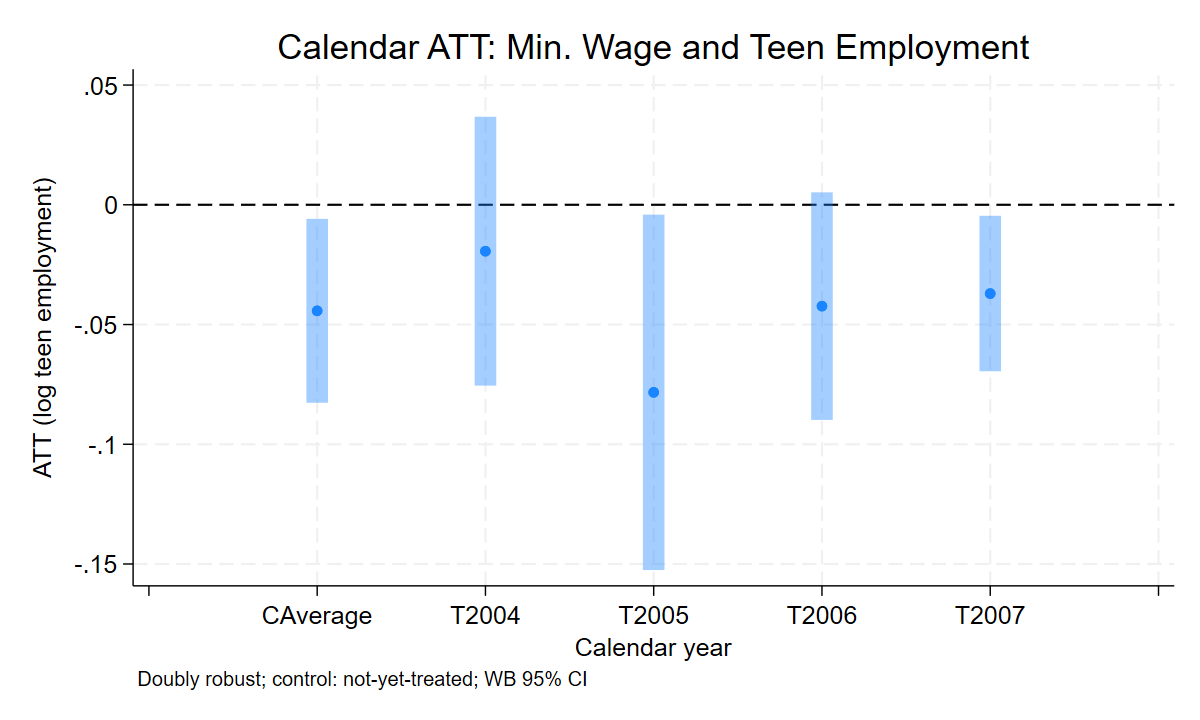
\includegraphics[width=\textwidth]{figures/cs/mpdta_calendar.png}
    \end{column}
    \begin{column}{0.42\textwidth}
      \small
      \textbf{Estimand: $\theta_c(t)$} --- average effect across cohorts
      already treated by calendar year $t$ (CAverage $=-0.044$).

      \medskip
      \textbf{2004--2005:} only the 2004 cohort is treated; its effect
      builds ($-0.02 \to -0.08$).

      \medskip
      \textbf{2006--2007:} the 2006 and 2007 cohorts (40 and 131
      counties, against 20 in 2004) enter with smaller effects and
      pull the average toward $-0.04$.

      \medskip
      \textbf{Use it} to ask: ``what was the average effect across all
      treated units in year $t$?'' --- aggregate policy impact in a
      given year.
    \end{column}
  \end{columns}

\end{frame}


% ── Closing checklist ────────────────────────────────────────────────────
\begin{frame}{C\&S in Practice: Checklist}

  \textbf{Before you run the code:}
  \begin{enumerate}
    \item Confirm treatment is \textbf{binary and absorbing}
    \item Decide on comparison group: never-treated (the default) or
      not-yet-treated (\texttt{notyet})
    \item Decide on estimator: doubly robust, \texttt{method(dripw)},
      the default in \texttt{csdid} and in R's \texttt{did}
    \item If groups differ on observables: add covariates to the model
    \item If few treated clusters: SEs and \texttt{wboot} unreliable
      (Roth et al.\ 2023, Sec.~5.1)
  \end{enumerate}

  \bigskip
  \textbf{After you run the code:}
  \begin{enumerate}
    \item \textbf{Inspect ATT$(g,t)$ grid:} do pre-treatment cells
      look like zero?
    \item \textbf{Plot the event study:} pre-periods near zero? Not
      proof of PT: report HonestDiD $\bar M$.
    \item \textbf{Check cohort-specific effects:} is there heterogeneity
      across cohorts? If yes, report it --- do not just report
      the overall ATT.
    \item \textbf{Compare to TWFE:} they can be close, but
      \alert{report C\&S either way}.
  \end{enumerate}

  \bigskip
  \textbf{Stata:} \texttt{csdid} + \texttt{drdid} from SSC.

\end{frame}

\end{document}
